\section[Le Memorie]{Le Memorie}
\label{sec:memory}
\sectionframe{images/covers/cover_sd_memory.png}{Le Memorie}	 


\subsection[Lo scopo delle memorie]{Lo scopo delle memorie}
\begin{frame}
	\frametitle{Lo scopo delle memorie}
	
	\begin{block}{Lo scopo delle memorie}
		La memoria, in informatica, è un elemento di un computer che ha il compito di garantire la \textbf{persistenza dei dati e/o delle istruzioni dei programmi}.\\\vspace{0.5em}
		Esistono diversi \textbf{tipi di memoria} e la loro realizzazione fisica dà vita a vari supporti di memorizzazione differenti tra loro.\\\vspace{0.5em}
		Noi ne approfondiremo alcune:
		
		\begin{itemize}
			\item I flip-flop
			\item La ROM
			\item La RAM
			\item La cache
			\item La memoria di massa
		\end{itemize}
		
	\end{block}
	
\end{frame}


\subsection[La memorie volatili e non volatili]{La memorie volatili e non volatili}
\begin{frame}
	\frametitle{La memorie volatili e non volatili}
	 
	\begin{block}{La memoria volatile}
		è una memoria che \textbf{necessita dell'alimentazione elettrica} continua al fine di \textbf{mantenere memorizzate le informazioni}. Questo tipo di memorie sono anche note come memorie temporanee.\\\vspace{0.5em}

		Le odierne memorie RAM (Random Access Memory), insieme alle nuove tecnologie in fase di sviluppo T-RAM, Z-RAM e TT-RAM, sono tutti esempi di memorie non fisse
	\end{block}
	
	\begin{block}{La memoria non volatile}
		è una tipologia di memoria in grado di \textbf{mantenere le informazioni anche quando non viene alimentata}.
	\end{block}
	
\end{frame}


\subsection[I flip-flop]{I flip-flop}
\begin{frame}
%	\frametitle{I flip-flop}
	
	\begin{block}{I flip-flop}
		Esistono diverse tecnologie per la realizzazione dei circuiti di memoria. Uno dei dispositivi elettronici più semplici per la memorizzazione dei bit è il \textbf{flip-flop}. Il flip-flop è una delle possibili implementazioni della \textbf{cella di memoria elementare} volatile. \\ Ricordiamo che il bit è la più piccola unità di informazione elettronica che possiamo memorizzare.
	\end{block}
	
	\begin{block}{I flip-flop SR (detti SR Latch)}
		Il \textbf{flip-flop SR}, noto anche come \textbf{SR Latch}, può essere considerato uno dei circuiti logici sequenziali più basilari possibili. Questo semplice flip-flop è fondamentalmente un dispositivo bistabile di memoria a un bit che ha due ingressi:
		\begin{itemize}
			\item \textbf{S}: che prende il nome di \textbf{set}, che imposta l'uscita a 1
			\item \textbf{R}: che prende il nome di \textbf{reset}, che imposta l'uscita a 0
		\end{itemize}
	\end{block}
	
\end{frame}


\subsubsection[Flip-flop SR - NOR Gate]{Flip-flop SR - NOR Gate}
\begin{frame}
	\frametitle{Flip-flop SR - NOR Gate}
	 
	\begin{figure}[!htbp] 
		\centering
		%\advance\leftskip-0.25cm
		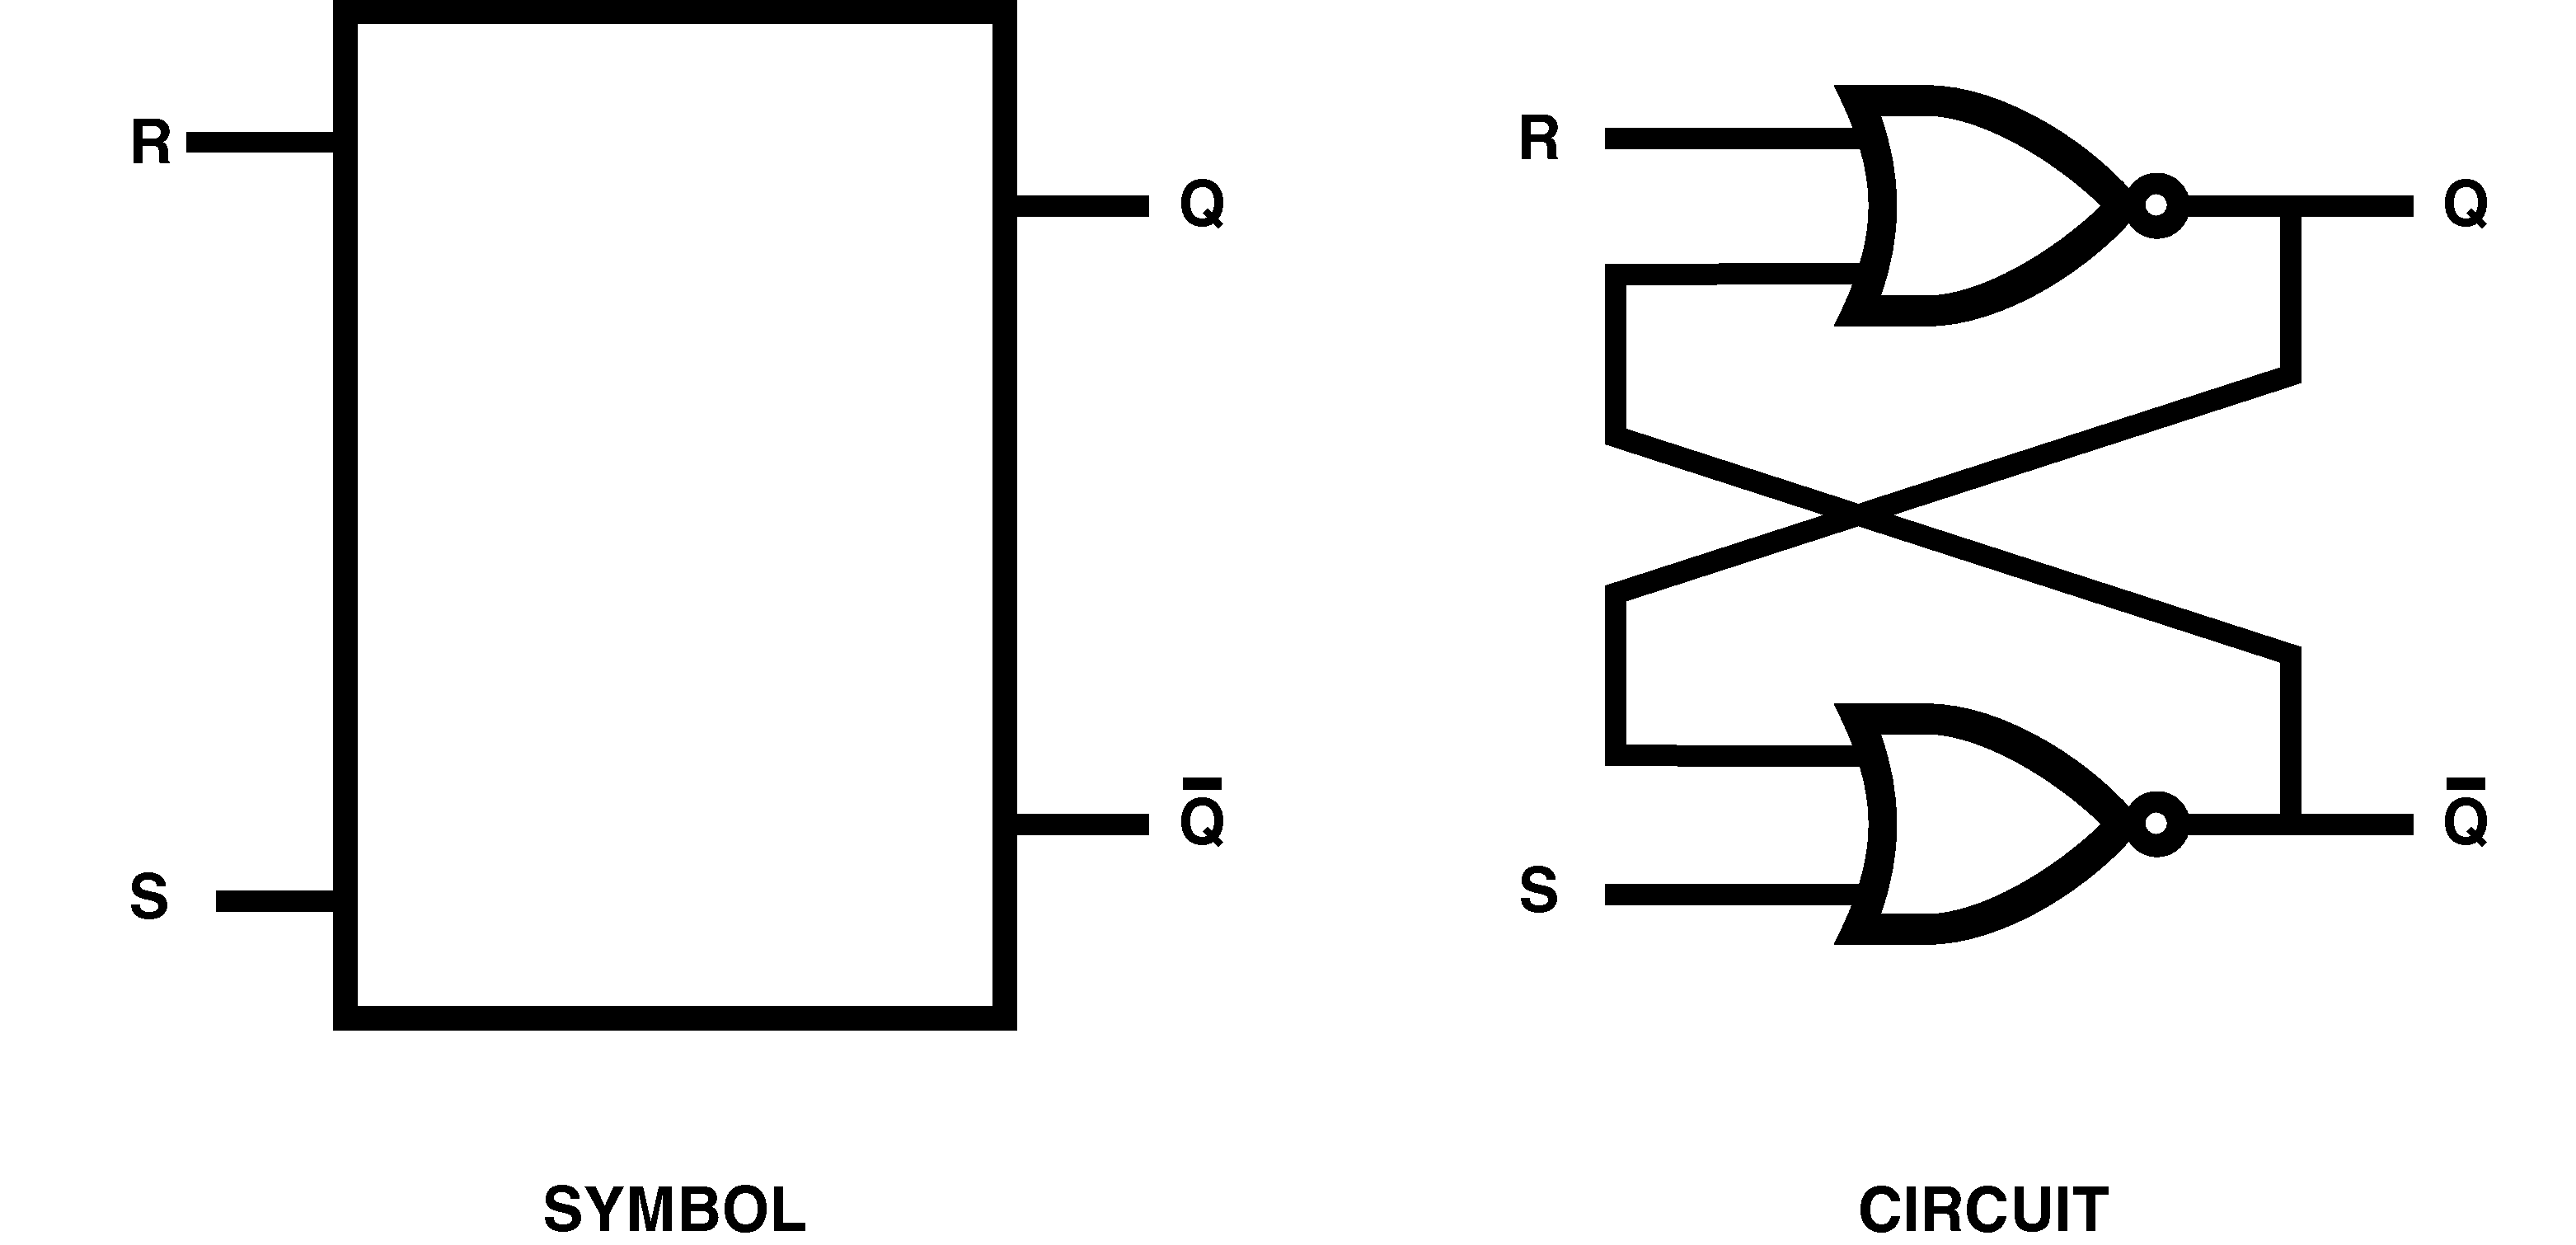
\includegraphics[width=0.95\linewidth]{images/5_memory/flip_flop_sr_nor.pdf}
		\caption{Il flip-flop SR: vedi il \underline{\href{https://www.youtube.com/watch?v=br2pbjAnP2k}{video su youtube}}}
	\end{figure}
	
\end{frame}

\begin{frame}
	\frametitle{Flip-flop SR - NOR Gate}
	 
	\begin{figure}[!htbp] 
		\centering
		%\advance\leftskip-0.25cm
		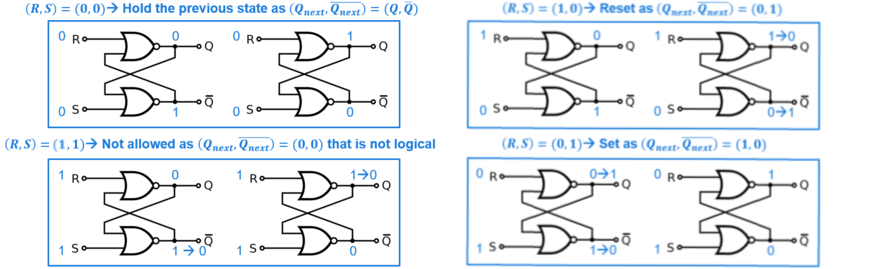
\includegraphics[width=1.0\linewidth]{images/5_memory/flip_flop_sr_nor.png}
		\caption{Il flip-flop SR con NOR, esempi}
	\end{figure}
	
\end{frame}

\begin{frame}

	\frametitle{Flip-flop SR - NOR Gate}

%	\begin{block}{K-means: algoritmo}
		\centering
		\animategraphics[controls={play, step, stop}, height=7cm]{3.0}{images/5_memory/flip_flop_sr_nor/flip_flop_sr_nor-}{0}{15}
		\label{fig:flip_flop_sr_nor}
%	\end{block}

\end{frame}


\subsubsection[Flip-flop SR - NAND Gate]{Flip-flop SR - NAND Gate}
\begin{frame}
	\frametitle{Flip-flop SR - NAND Gate}
	 
	\begin{figure}[!htbp]  
		\centering
		%\advance\leftskip-0.25cm
		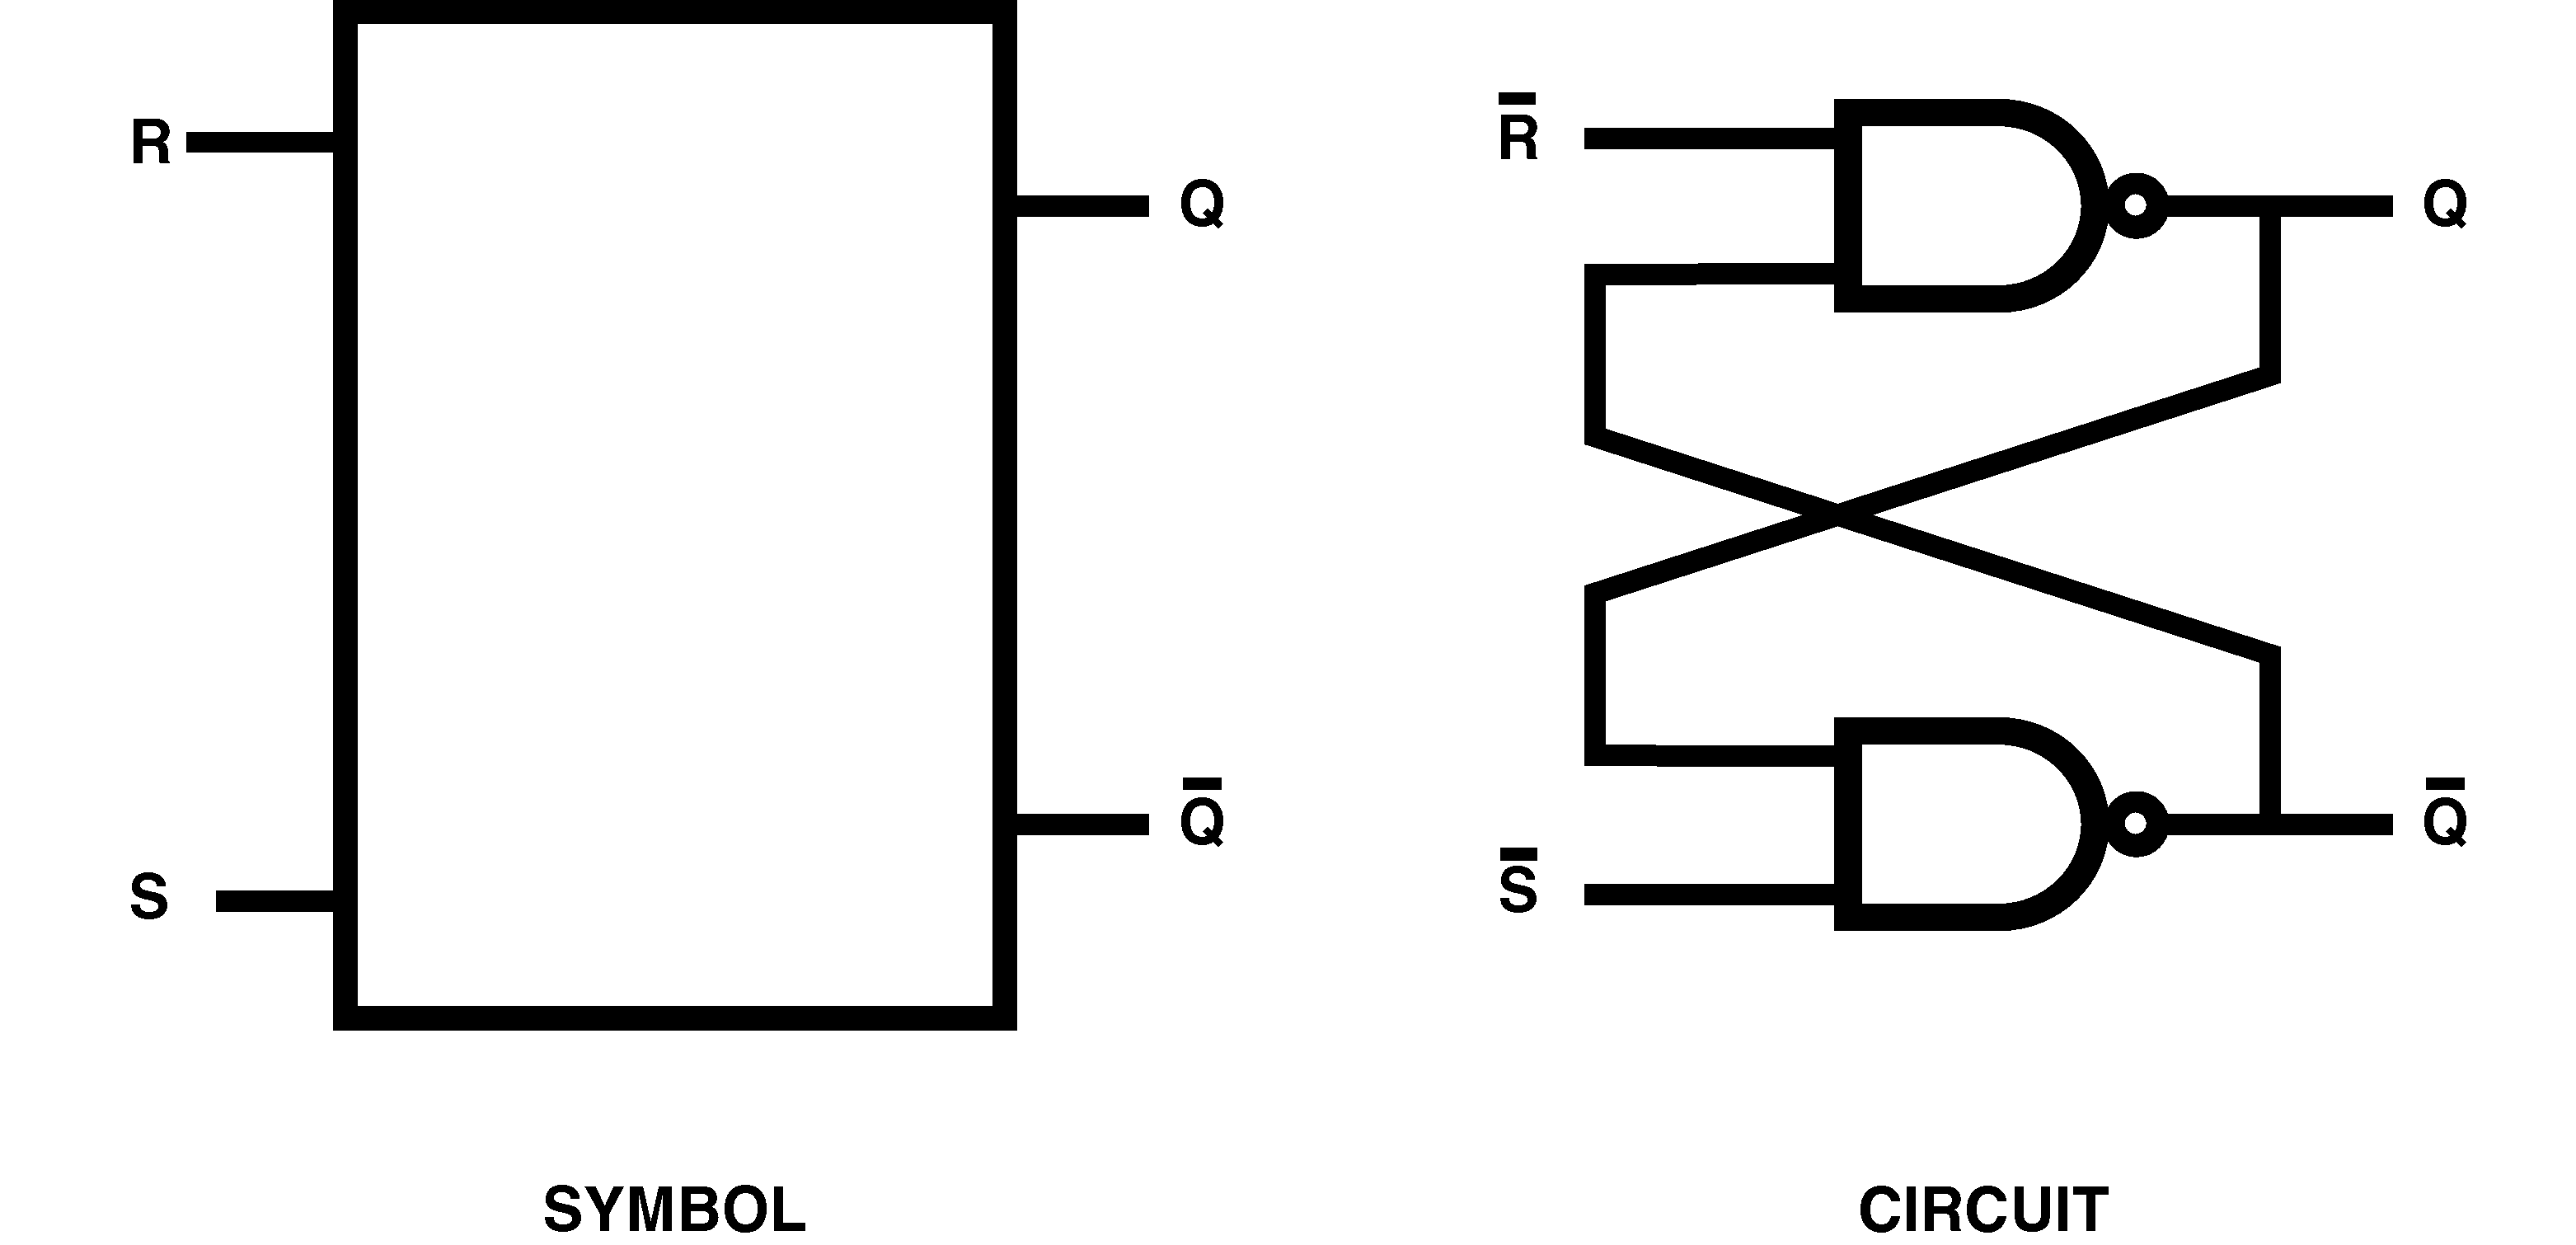
\includegraphics[width=0.95\linewidth]{images/5_memory/flip_flop_sr_nand.pdf}
		\caption{Il flip-flop SR: vedi il \underline{\href{https://www.youtube.com/watch?v=Y9k2oiSJkz4}{video su youtube}}}
	\end{figure}
	
\end{frame}


\subsubsection[Flip-flop D]{Flip-flop D}
\begin{frame}
	\frametitle{Flip-flop D}
	 
	\begin{figure}[!htbp] 
		\centering
		%\advance\leftskip-0.25cm
		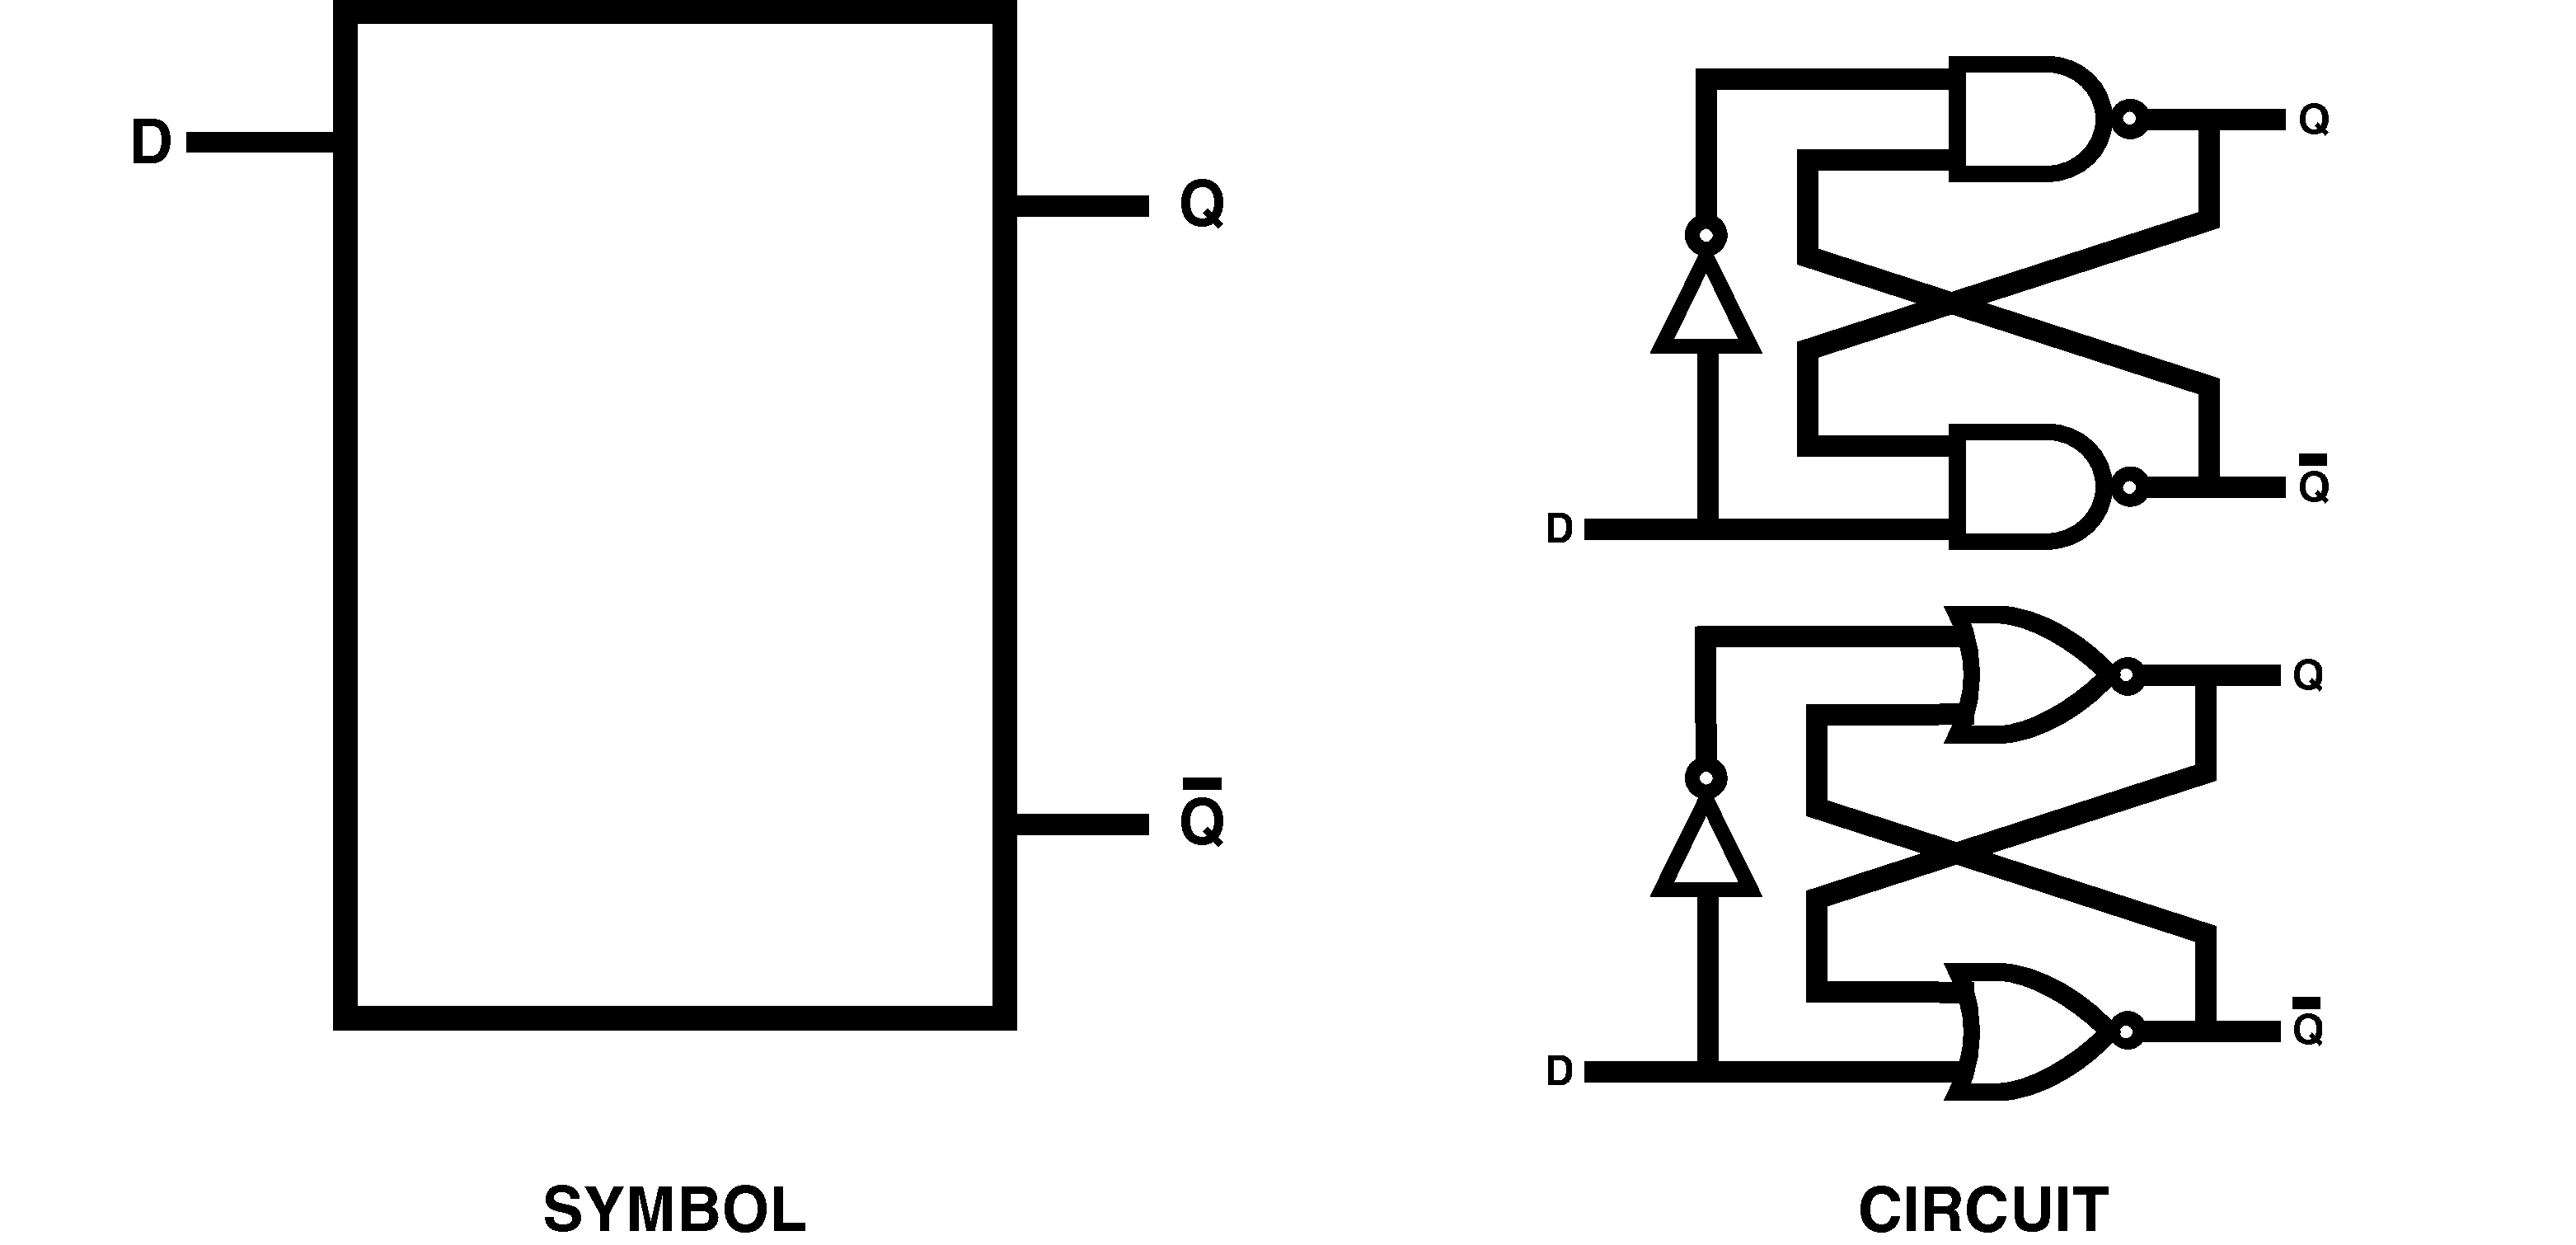
\includegraphics[width=0.75\linewidth]{images/5_memory/flip_flop_d.pdf}
		\caption{Il flip-flop D: è utile per memorizzare un bit di informazione che vengono presentate su una sola line detta "\textbf{Data Line}" (da cui la lettera \textbf{D})}
	\end{figure}
	
\end{frame}




\subsection[La ROM (Read Only Memory)]{La ROM (Read Only Memory)}
\begin{frame}
	\frametitle{La ROM (Read Only Memory)}
	  
	\begin{block}{La ROM (Read Only Memory)}
		In elettronica e informatica, una memoria di sola lettura, meglio nota come \textbf{ROM (Read Only Memory)}, indica un tipo di memoria \textit{non volatile} in cui i dati sono memorizzati tramite collegamenti elettronici fisici e stabili.
		
		\begin{figure}[!htbp] 
			\centering
			%\advance\leftskip-0.25cm
			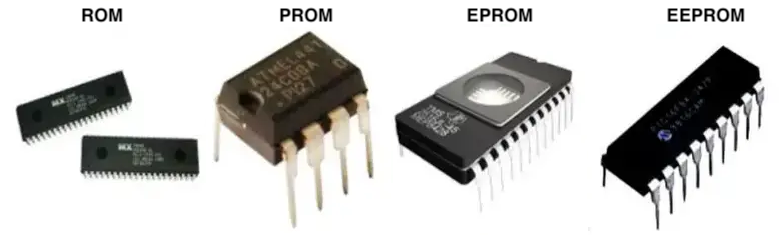
\includegraphics[width=0.80\linewidth]{images/5_memory/roms.png}
			%\caption{Il flip-flop D: è utile per memorizzare un bit di informazione che vengono presentate su una sola line detta "\textbf{Data Line}" (da cui la lettera \textbf{D})}
		\end{figure}
		
		Nonostante il nome suggerisca diversamente alcune ROM possono essere riscritte se sottoposte a specifiche condizioni fisiche.
		
		
		%Contrariamente alla maggior parte delle unità di memoria di massa il suo contenuto non è modificabile durante il normale funzionamento, ma può esserlo, con diverse tecniche, in fase di progettazione, prototipazione o costruzione.
	\end{block}
	
\end{frame}


\begin{frame}
	\frametitle{Le tipologie di ROM}
	  
	\begin{block}{Le tipologie di ROM}
		
		Ogni tipo di ROM è programmata in modo differente a seconda del suo tipo e richiede condizioni speciali per essere cancellata o riscritta.
		
		\begin{figure}[!htbp] 
			\centering
			%\advance\leftskip-0.25cm
			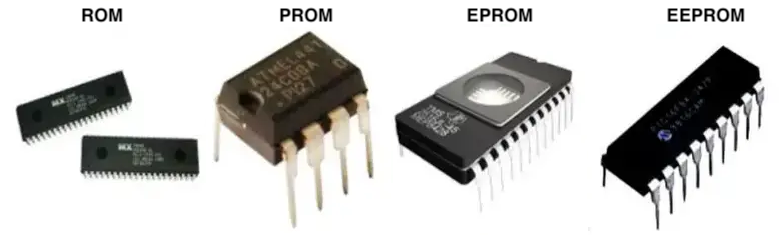
\includegraphics[width=0.80\linewidth]{images/5_memory/roms.png}
			%\caption{Il flip-flop D: è utile per memorizzare un bit di informazione che vengono presentate su una sola line detta "\textbf{Data Line}" (da cui la lettera \textbf{D})}
		\end{figure}
		
		Le  memorie ROM vengono in genere utilizzate per memorizzare programmi e dati di configurazione essenziali per il funzionamento del computer che devono essere memorizzati anche quando il computer è spento.
	\end{block}
	
\end{frame}


\begin{frame}
	\frametitle{Le tipologie di ROM: non programmabili}
	  
	\begin{block}{}
		
		\begin{enumerate}
			\item \textbf{ROM non programmabili}: ROM a maschera, il cui nome deriva dal processo di litografia utilizzato nei circuiti integrati (chip), in cui una fotomaschera permette la creazione del chip. Vengono prodotte già con il programma o i dati "stampati" al loro interno.
		\end{enumerate}
	\end{block}
	
	\begin{columns}			
		\column{0.5\linewidth}
		\begin{figure}[!htbp]
			\centering 
			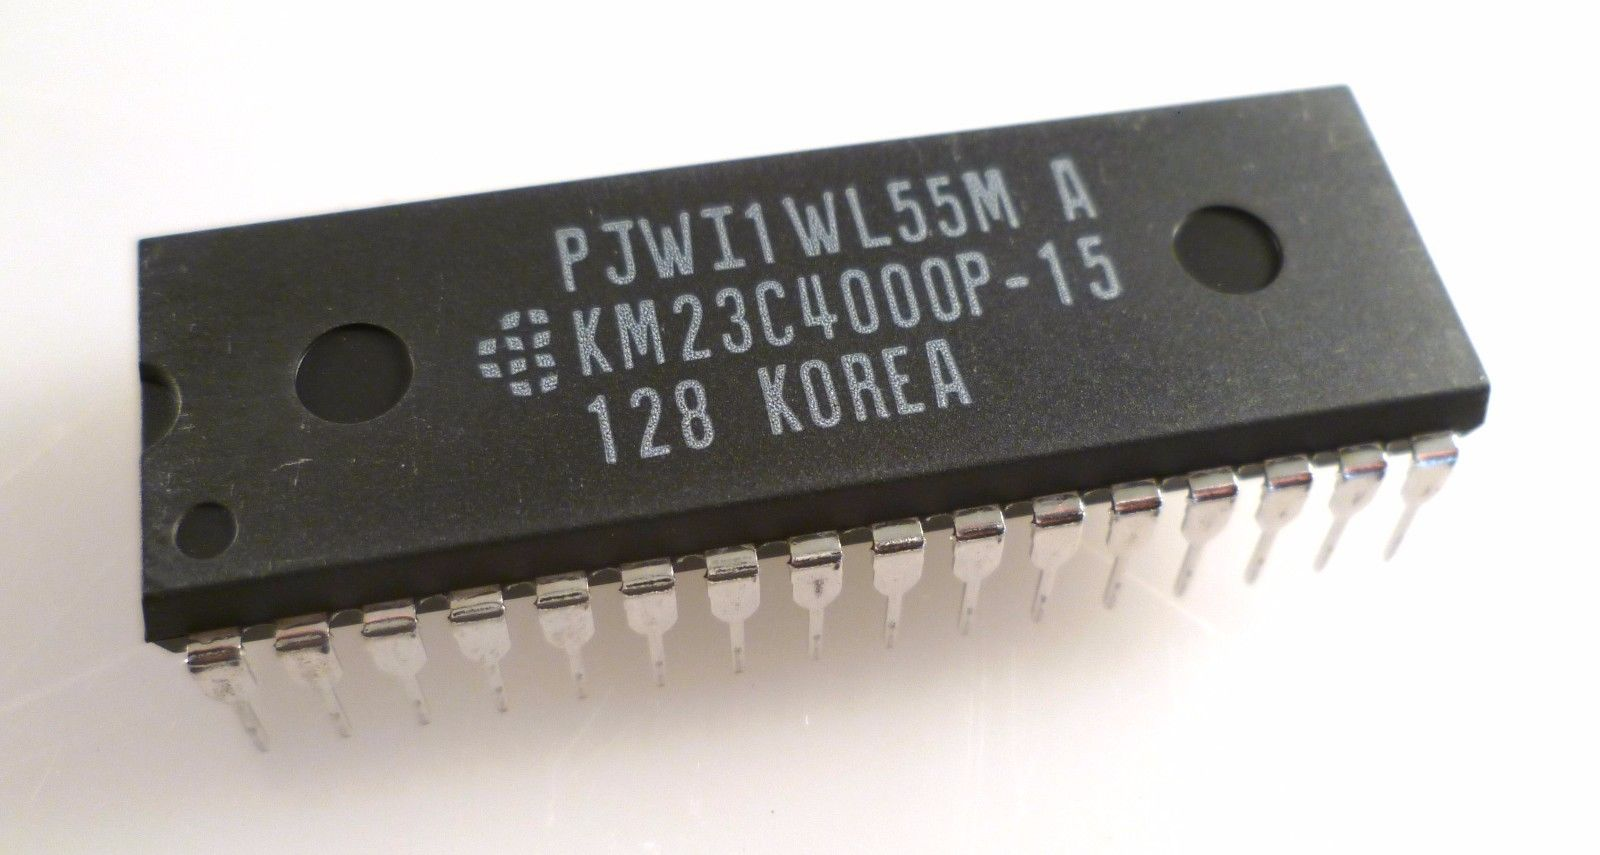
\includegraphics[width=1.0\linewidth]{images/5_memory/rom_mask_top.jpeg}
%				\caption{ROM a maschera}
		\end{figure}
		
		\column{0.5\linewidth}
		\begin{figure}[!htbp]
			\centering 
			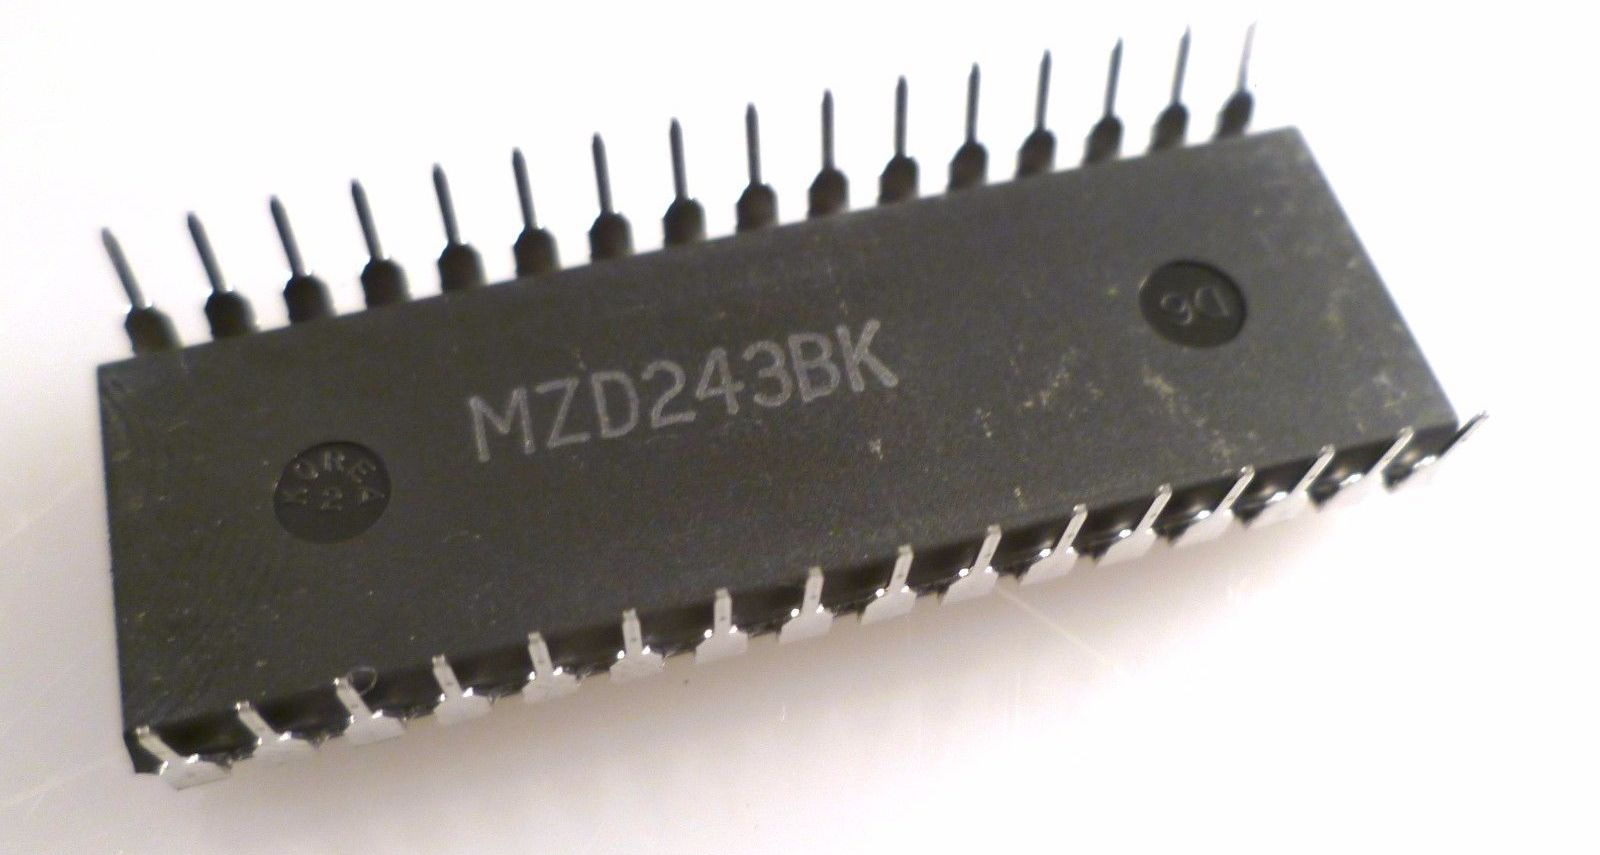
\includegraphics[width=1.0\linewidth]{images/5_memory/rom_mask_bottom.jpeg}
%				\caption{PCI Express: x16, x1, x4, x16} 
		\end{figure}
	\end{columns}
	
\end{frame}


\begin{frame}
	\frametitle{Le tipologie di ROM: PROM}
	  
	\begin{block}{}
		
		\begin{enumerate}
			\setcounter{enumi}{1}
			\item \textbf{PROM  (Programmable  ROM)}: normalmente vengono prodotte vuote al loro interno, possono essere programmate successivamente attraverso appositi \textbf{programmatori di PROM},  tuttavia, una volta programmate, non possono essere più modificate nel  contenuto.
		\end{enumerate}
	\end{block}
	
	\begin{figure}[!htbp] 
		\centering
		%\advance\leftskip-0.25cm
		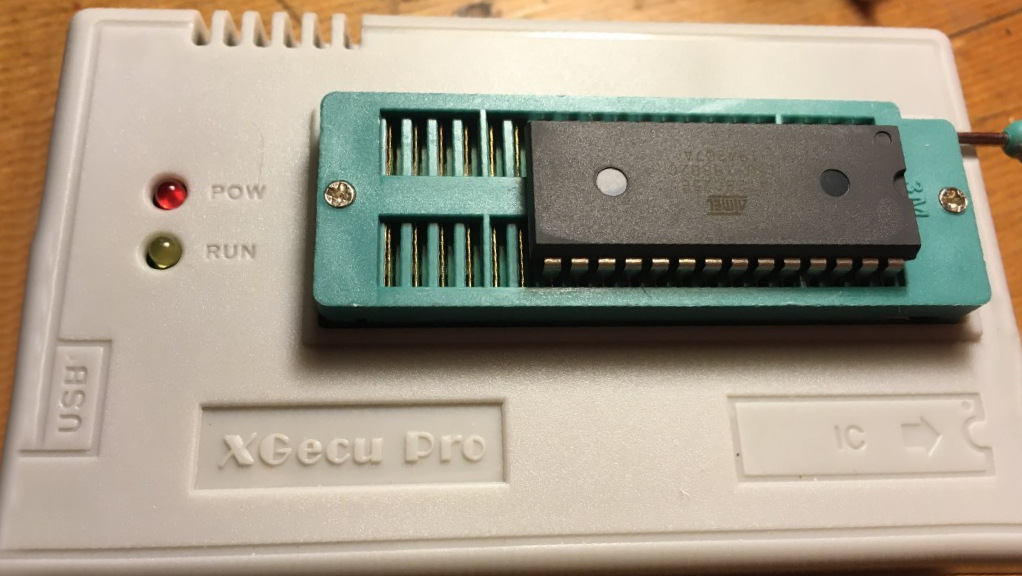
\includegraphics[width=0.7\linewidth]{images/5_memory/prom_programmer.png}
		%\caption{Programmatore di PROM}
	\end{figure}
	
\end{frame}


\begin{frame}
	\frametitle{Le tipologie di ROM: EPROM}
	  
	\begin{block}{}

		\begin{enumerate}
			\setcounter{enumi}{2}
			\item \textbf{EPROM (Erasable Programmable ROM)}: normalmente sono vuote al loro interno e possono  essere  programmate  attraverso appositi programmatori di EPROM. A differenza delle PROM, la programmazione può avvenire più volte, a patto di cancellare la vecchia programmazione tramite raggi UV (ultravioletti).
		\end{enumerate}
		
	\end{block}
	
	\begin{columns}			
		\column{0.5\linewidth}
		\begin{figure}[!htbp]
			\centering 
			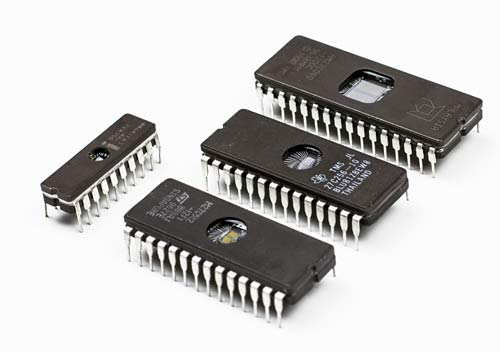
\includegraphics[width=1.0\linewidth]{images/5_memory/eproms.jpg }
%				\caption{ROM a maschera}
		\end{figure}
		
		\column{0.5\linewidth}
		\begin{figure}[!htbp]
			\centering 
			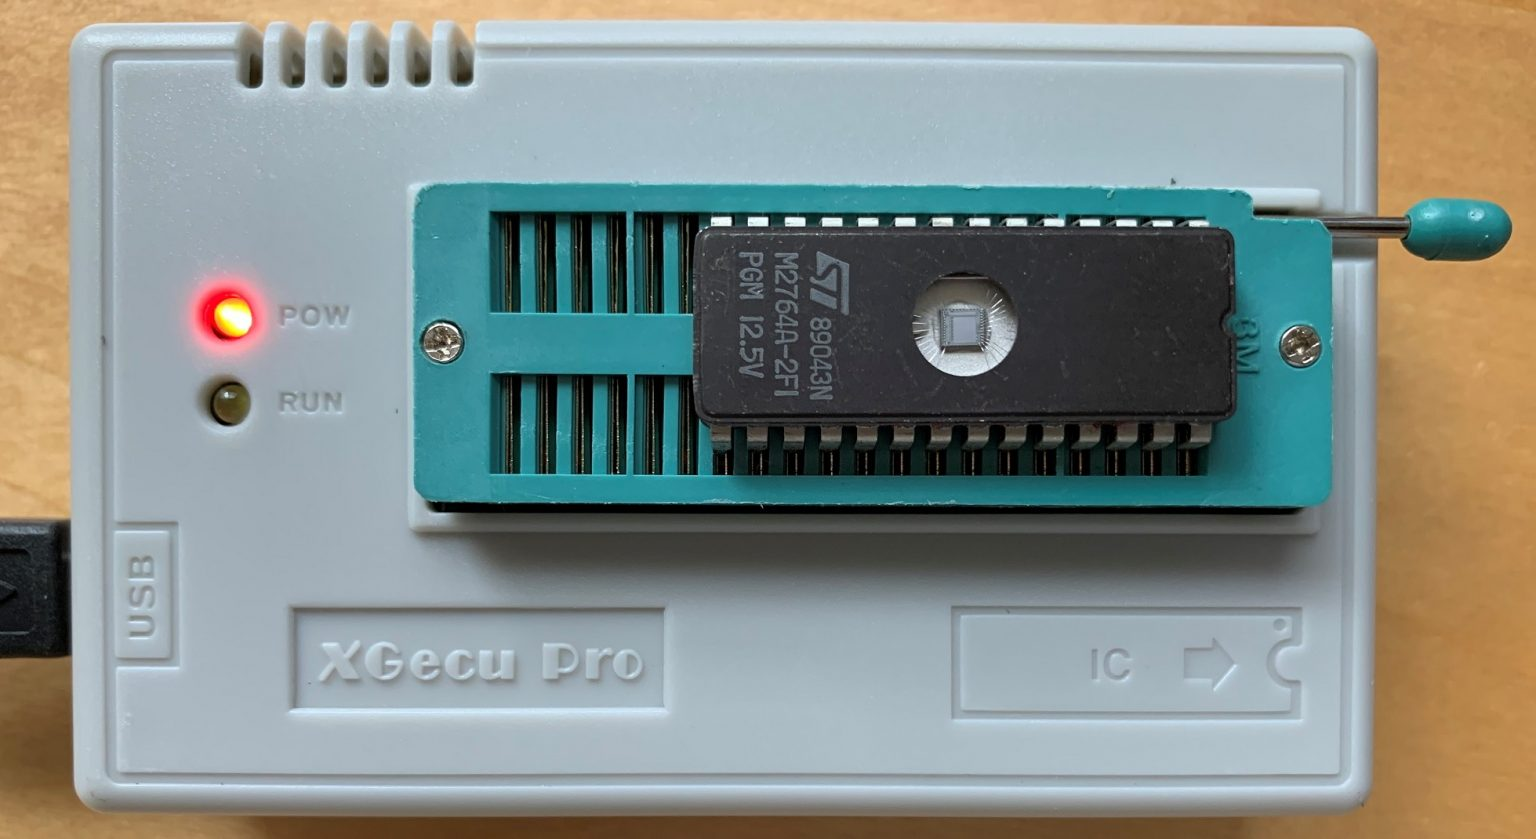
\includegraphics[width=1.0\linewidth]{images/5_memory/eprom_programmer.jpg}
%				\caption{PCI Express: x16, x1, x4, x16} 
		\end{figure}
	\end{columns}
	
	\begin{figure}[!htbp] 
		\centering
		%\advance\leftskip-0.25cm
		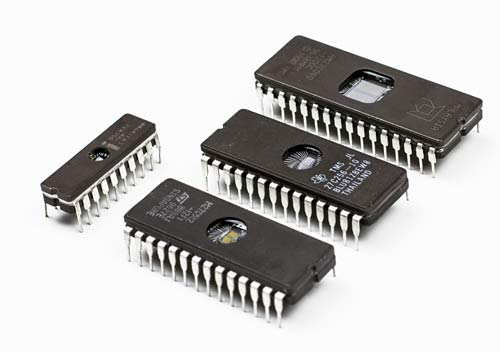
\includegraphics[width=0.5\linewidth]{images/5_memory/eproms.jpg }
		%\caption{PROM: nota la finestrella posta nella parte superiore del  circuito, che permette di ricevere i raggi UV}
	\end{figure}
	
\end{frame}


\begin{frame}
	\frametitle{Le tipologie di ROM: EPROM}
	 
	\begin{figure}[!htbp] 
		\centering
		%\advance\leftskip-0.25cm
		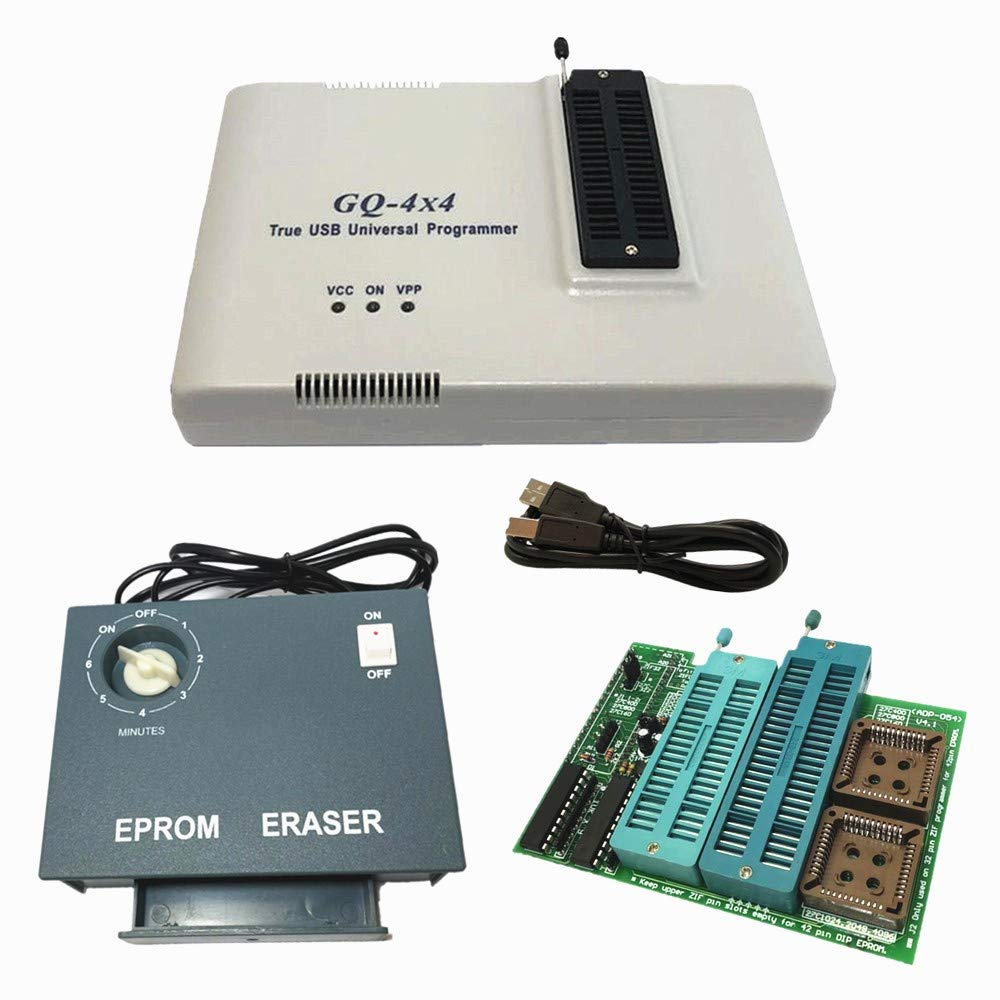
\includegraphics[width=0.6\linewidth]{images/5_memory/eprom_writer_eraser.jpg}
		%\caption{PROM: nota la finestrella posta nella parte superiore del  circuito, che permette di ricevere i raggi UV}
	\end{figure}
	
\end{frame}


\begin{frame}
	\frametitle{Le tipologie di ROM: EPROM}
	 
	\begin{figure}[!htbp] 
		\centering
		%\advance\leftskip-0.25cm
		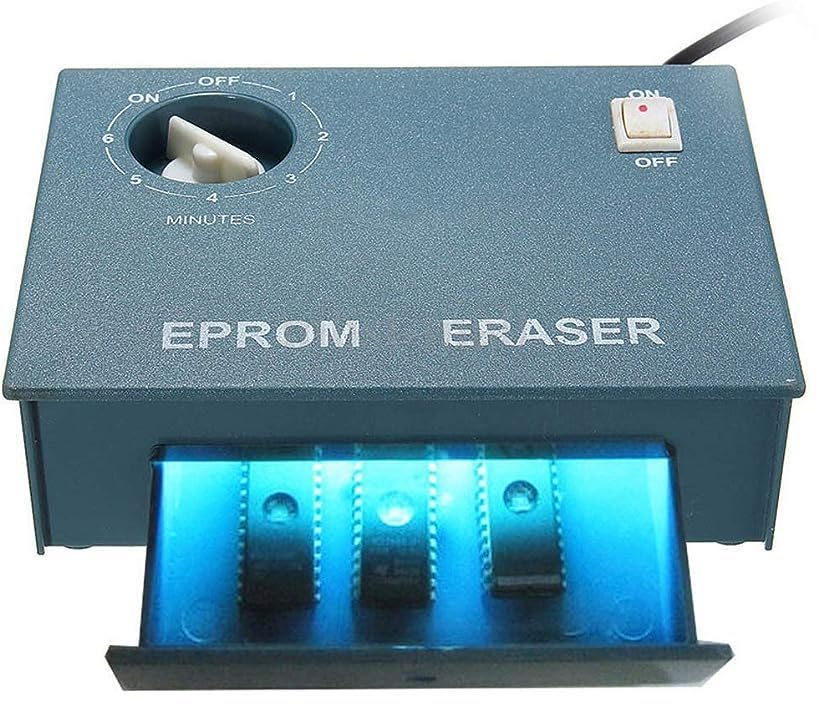
\includegraphics[width=0.6\linewidth]{images/5_memory/eprom_eraser.jpg}
		%\caption{PROM: nota la finestrella posta nella parte superiore del  circuito, che permette di ricevere i raggi UV}
	\end{figure}
	
\end{frame}




\begin{frame}
	\frametitle{Le tipologie di ROM: EEPROM}
	  
	\begin{block}{}

		\begin{enumerate}
			\setcounter{enumi}{3}
			\item \textbf{EEPROM (Electrical  Erasable  Programmable  ROM)}: identiche alle EPROM, dalle quali differiscono solo per il fatto che la cancellazione della vecchia programmazione è realizzata più semplicemente tramite un flusso di corrente elettrica. 
		\end{enumerate}
		
	\end{block}
	
	\begin{figure}[!htbp] 
		\centering
		%\advance\leftskip-0.25cm
		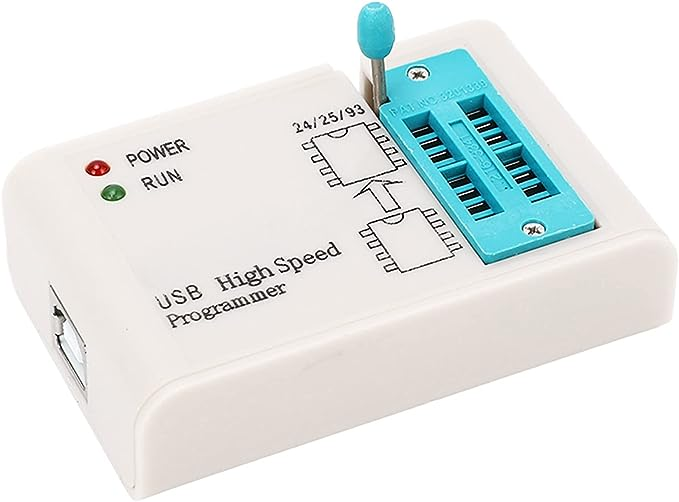
\includegraphics[width=0.55\linewidth]{images/5_memory/eeprom_programmer.jpg}
		%\caption{Programmatore di PROM}
	\end{figure}
	
\end{frame}




\subsection[Il collo di bottiglia delle memorie]{Il collo di bottiglia delle memorie}
\begin{frame}
	\frametitle{Il collo di bottiglia delle memorie}
	 
	\begin{block}{Il collo di bottiglia}
		Il \textbf{collo di bottiglia} è un fenomeno che si verifica quando le prestazioni di un sistema o le sue capacità sono fortemente vincolate da un singolo componente. Il termine è una metafora del collo di bottiglia reale, che limita il flusso d'uscita dell'acqua.
	\end{block}
	
	\begin{block}{Le prestazioni della memoria RAM}
		Le prestazioni della CPU si sono evolute nel tempo e le prestazioni sono aumentate in maniera esponenziale (vedi \textbf{Legge di Moore}).\\
		Le prestazioni delle memorie non riuscite a tenere il passo con tale ritmo, per questo è stato necessario trovare delle strategie per ridurre al minimo l'impatto di tale collo di bottiglia.
	\end{block}
	
\end{frame}


\subsection[La gerarchia delle memorie]{La gerarchia delle memorie}
\begin{frame}
	\frametitle{Il collo di bottiglia delle memorie}
	 
	\begin{block}{Le prestazioni della memoria RAM}
		Una delle strategie adottate per migliorare le prestazioni consiste nel combinare tipi di memoria veloce con tipi di memoria più capienti ma lente: un sistema gerarchico di memorie.
	\end{block}
	
	\begin{figure}[!htbp] 
		\centering
		%\advance\leftskip-0.25cm
		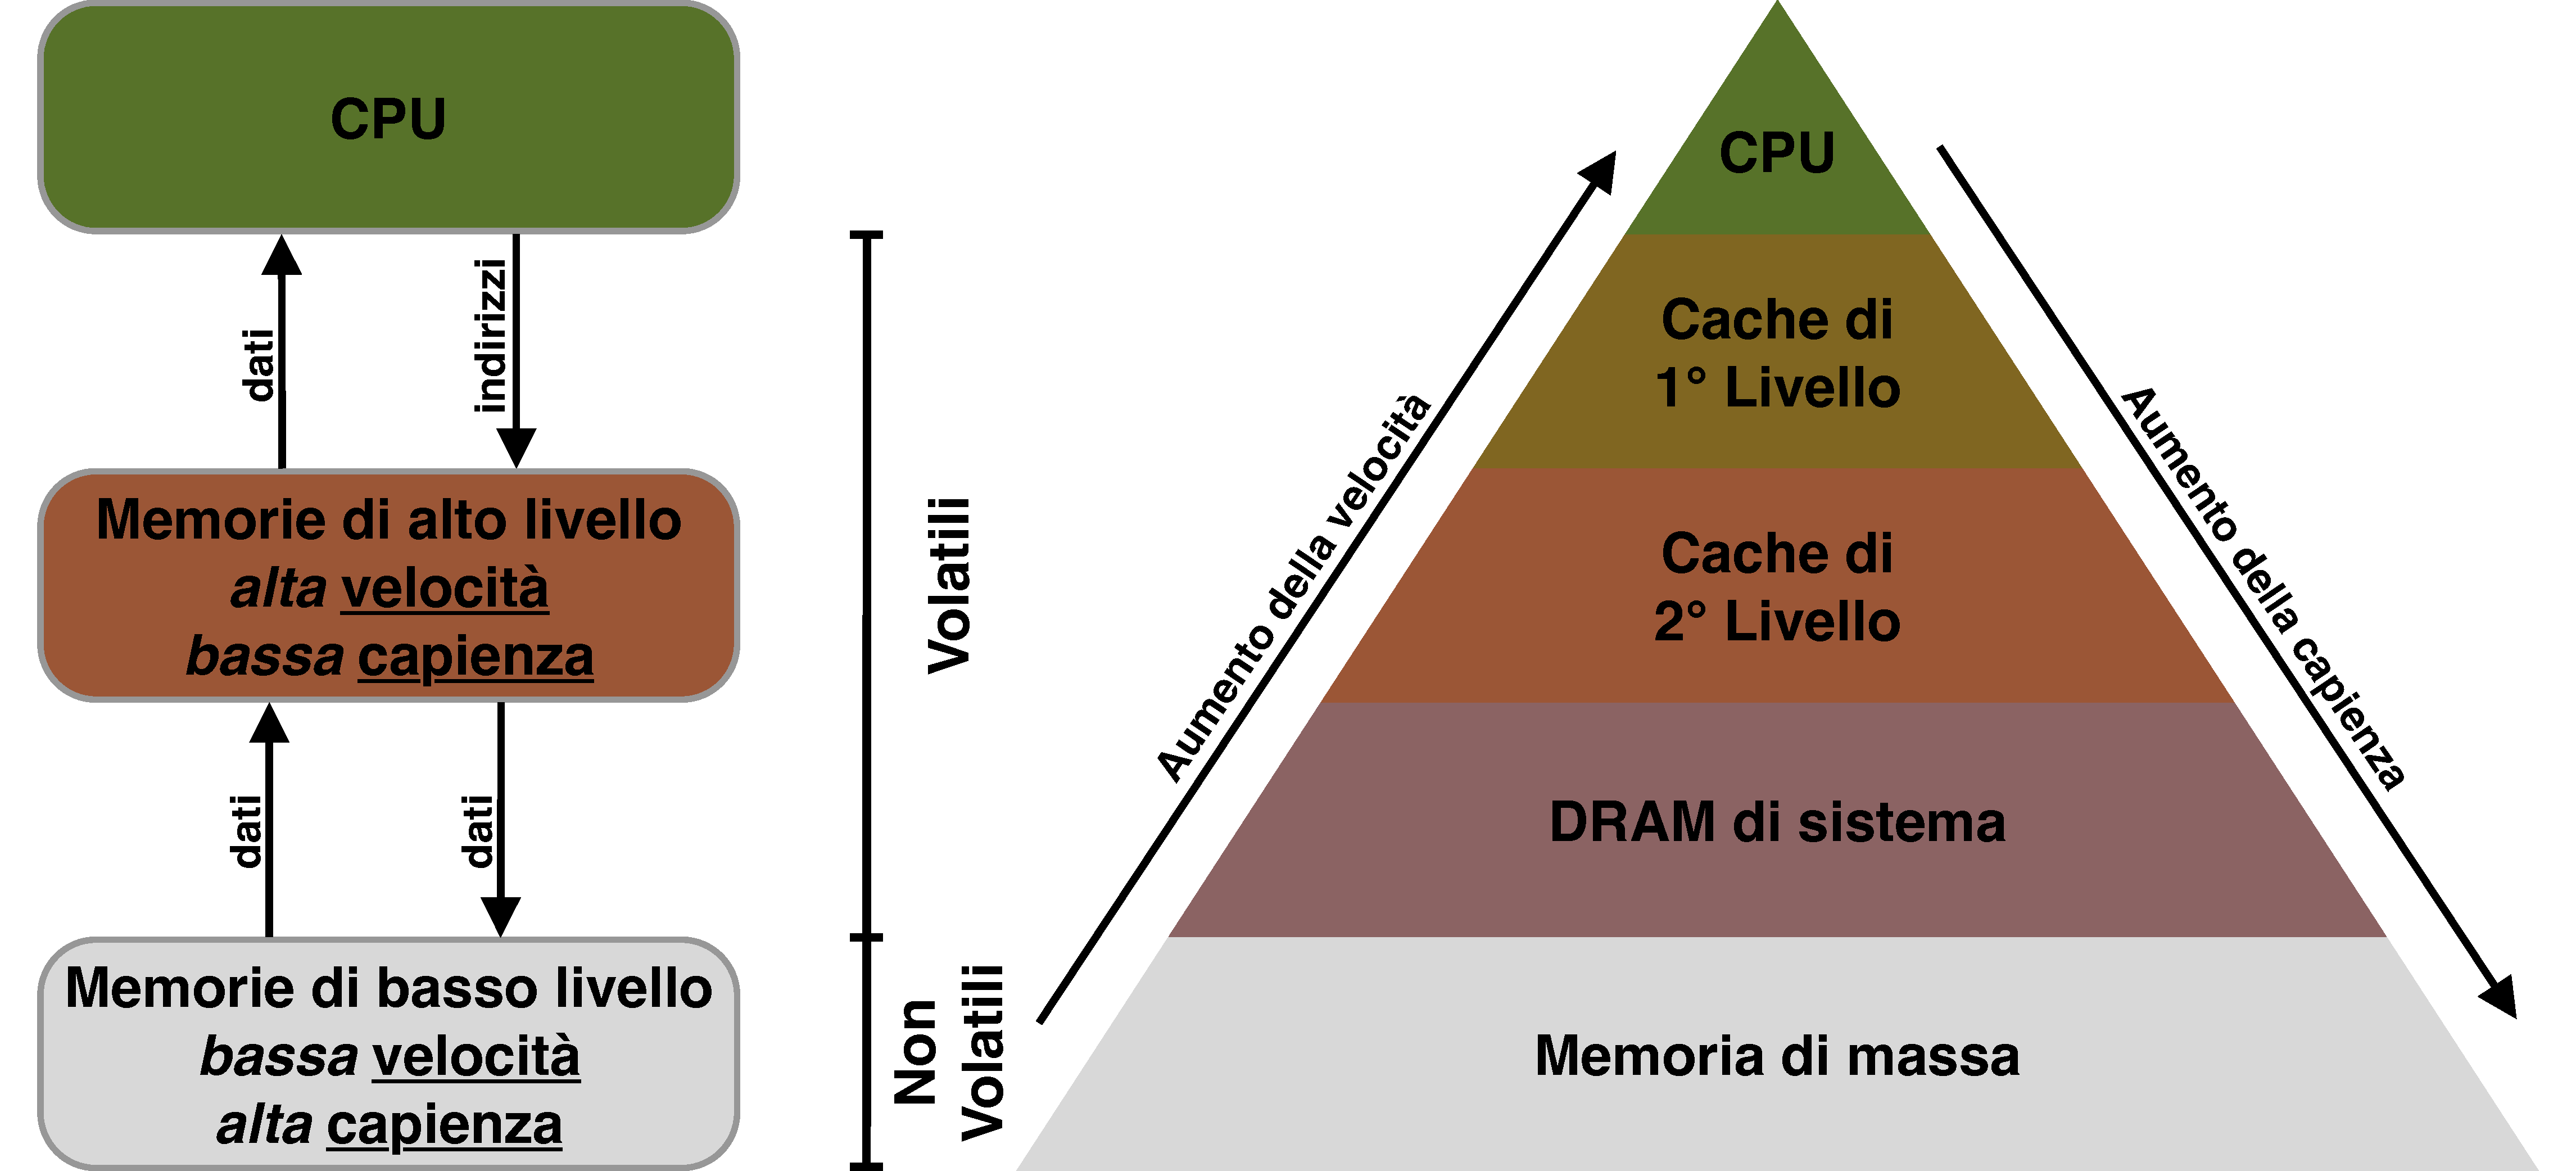
\includegraphics[width=0.8\linewidth]{images/5_memory/memory_hierarchy.pdf}
%		\caption{La CPU: CU, ALU e registri}
		\label{fig:memory_hierarchy}
	\end{figure} 

\end{frame}